\documentclass[12pt, a4paper]{article}
\usepackage[utf8]{inputenc}
\usepackage[english]{babel}
\usepackage{amsmath}
\usepackage{amsfonts}
\usepackage{amssymb}
\usepackage{csquotes}
\usepackage{mathtools}
\usepackage{graphicx}
\usepackage{geometry}
\usepackage{setspace}
\usepackage{longtable}
\usepackage{float}
\usepackage{comment}
\usepackage{listings}
\usepackage{enumerate}
\usepackage{enumitem}
\usepackage[colorlinks=true, allcolors=blue]{hyperref}

\usepackage[style=authoryear]{biblatex}
\addbibresource{Bibliography.bib}
\lstset{language=Python,
    showstringspaces=false,
    showtabs=false}

\geometry{top = 2.5cm, bottom = 2.5cm, left= 3cm, right= 3cm}

\title{Determination of Planck's Constant}
\author{Lee Farrugia \\ Experiment 15 \\ Group 1A}

\date{$6^{\text{th}}$ December 2021}

\begin{document}

\maketitle

\section*{Aim}
The aim of this experiment is to determine Planck's constant through the use of the photoelectric effect. 

\section*{Diagram}
\begin{figure}[H]
    \centering
    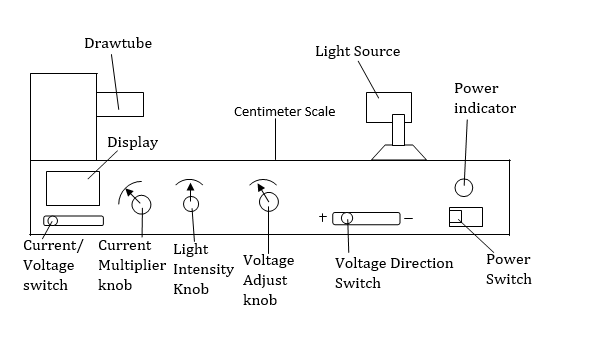
\includegraphics{Experiment 15 Diagram.png}
    \caption{Apparatus Diagram}
    \label{fig:Diagram}
\end{figure}

\section*{List of Apparatus}
Light source, Narrow band pass filters, Unknown metal, Drawtube

\section*{Language and Packages}
Python 3.9.7, Numpy, Matplotlib.pyplot, Pandas

\section*{Procedure}
\begin{enumerate}
    \item The light source was positioned at the 36 cm mark on the centimeter scale on the top of the apparatus.
    \item The apparatus was switched on and left to heat up, which took around 5 minutes.
    \item The red colour filter was inserted into the drawtube.
    \item The Current/Voltage switch was set so that the voltage was shown. 
    \item The voltage direction was set to negative.
    \item The voltage adjust knob was rotated anticlockwise until the voltage was around 0 V.
    \item The Current/Voltage switch was set so that the current is shown.
    \item The current multiplier was set to ``$\times0.001$".
    \item The light intensity was varied by adjusting the light intensity knob until the current on the display was about 0.3 \textmu A. It was taken care that the maximum value of the ammeter scale of 2 \textmu A. This setting was kept for the rest of the experiment.
    \item The light source was moved forward. The change in the photoelectric current was noted.
    \item The light source was placed in its original position.
    \item The voltage adjusting knob was rotated until the photocurrent was zero. This was called stopping voltage and was noted in the table below.
    \item The Current/Voltage switch was set so that the voltage was shown. 
    \item The light source was moved forward and any change in the voltage value was noted.
    \item The wavelength of the filter was noted in the table below.
    \item The stopping voltages of the other filters were also determined using the previous four steps.
\end{enumerate}

\section*{Precautions}
\begin{itemize}
    \item[-] The apparatus was left untouched until the indicator light had turned on, which meant that the bulb had heated up.
    \item[-] The original position was used for all of the different filters.
    \item[-] The maximum 2 \textmu A value of current was not exceeded. 
    \item[-] Repeated readings of the stopping voltage were taken.
    \item[-] When reading the stopping voltage, the bulb was moved in order to confirm that there was no fluctuation of the value.
\end{itemize}

\section*{Sources of Error}
\begin{itemize}
    \item[-] For small values of current the apparatus was fluctuating readings randomly.
    \item[-] The values of voltage and current might not have been 0 V , 0 \textmu A respectively.
    \item[-] Due to the amount of steps in the procedure the apparatus was left turned on for a long period of time, thus the temperature of the bulb had increased more.
    \item[-] The moving of the bulb in the first part of the procedure might have resulted in the bulb moving vertically as well.
    \item[-] The experiment was not done in a dark room, thus introducing some minor inaccuracies.
\end{itemize}

\section*{Data and Graphs}
\begin{longtable}{|c|c|}
\caption{Filter colour and its wavelength}
\label{tab:Table 1}\\ \hline
filter colour & wavelength/m    \\ \hline
\endfirsthead

\endhead

red     & $6.35\times10^{-7}$ \\ \hline
orange  & $5.70\times10^{-7}$ \\ \hline
yellow  & $5.40\times10^{-7}$ \\ \hline
green   & $5.00\times10^{-7}$ \\ \hline
blue    & $4.60\times10^{-7}$ \\ \hline
\end{longtable}

\begin{longtable}{|c|c|c|c|c|}
\caption{Filter colour and Stopping Voltage}
\label{tab:Table 2}\\ \hline
svred & svorange & svyellow & svgreen & svblue \\ \hline
\textpm 0.01 & \textpm 0.01 & \textpm 0.01 & \textpm 0.01 & \textpm 0.01 \\ \hline
\endfirsthead

\hline svred & svorange & svyellow & svgreen & svblue \\ \hline
\textpm 0.01 & \textpm 0.01 & \textpm 0.01 & \textpm 0.01 & \textpm 0.01 \\ \hline
\endhead

$-0.36$ & $-0.58$ & $-0.75$ & $-0.90$ & $-1.05$  \\ \hline
$-0.36$ & $-0.58$ & $-0.75$ & $-0.91$ & $-1.06$  \\ \hline
$-0.35$ & $-0.58$ & $-0.75$ & $-0.90$ & $-1.05$  \\ \hline 
$-0.35$ & $-0.58$ & $-0.75$ & $-0.91$ & $-1.07$  \\ \hline
$-0.36$ & $-0.58$ & $-0.75$ & $-0.92$ & $-1.06$  \\ \hline
\end{longtable}

\begin{figure}
    \centering
    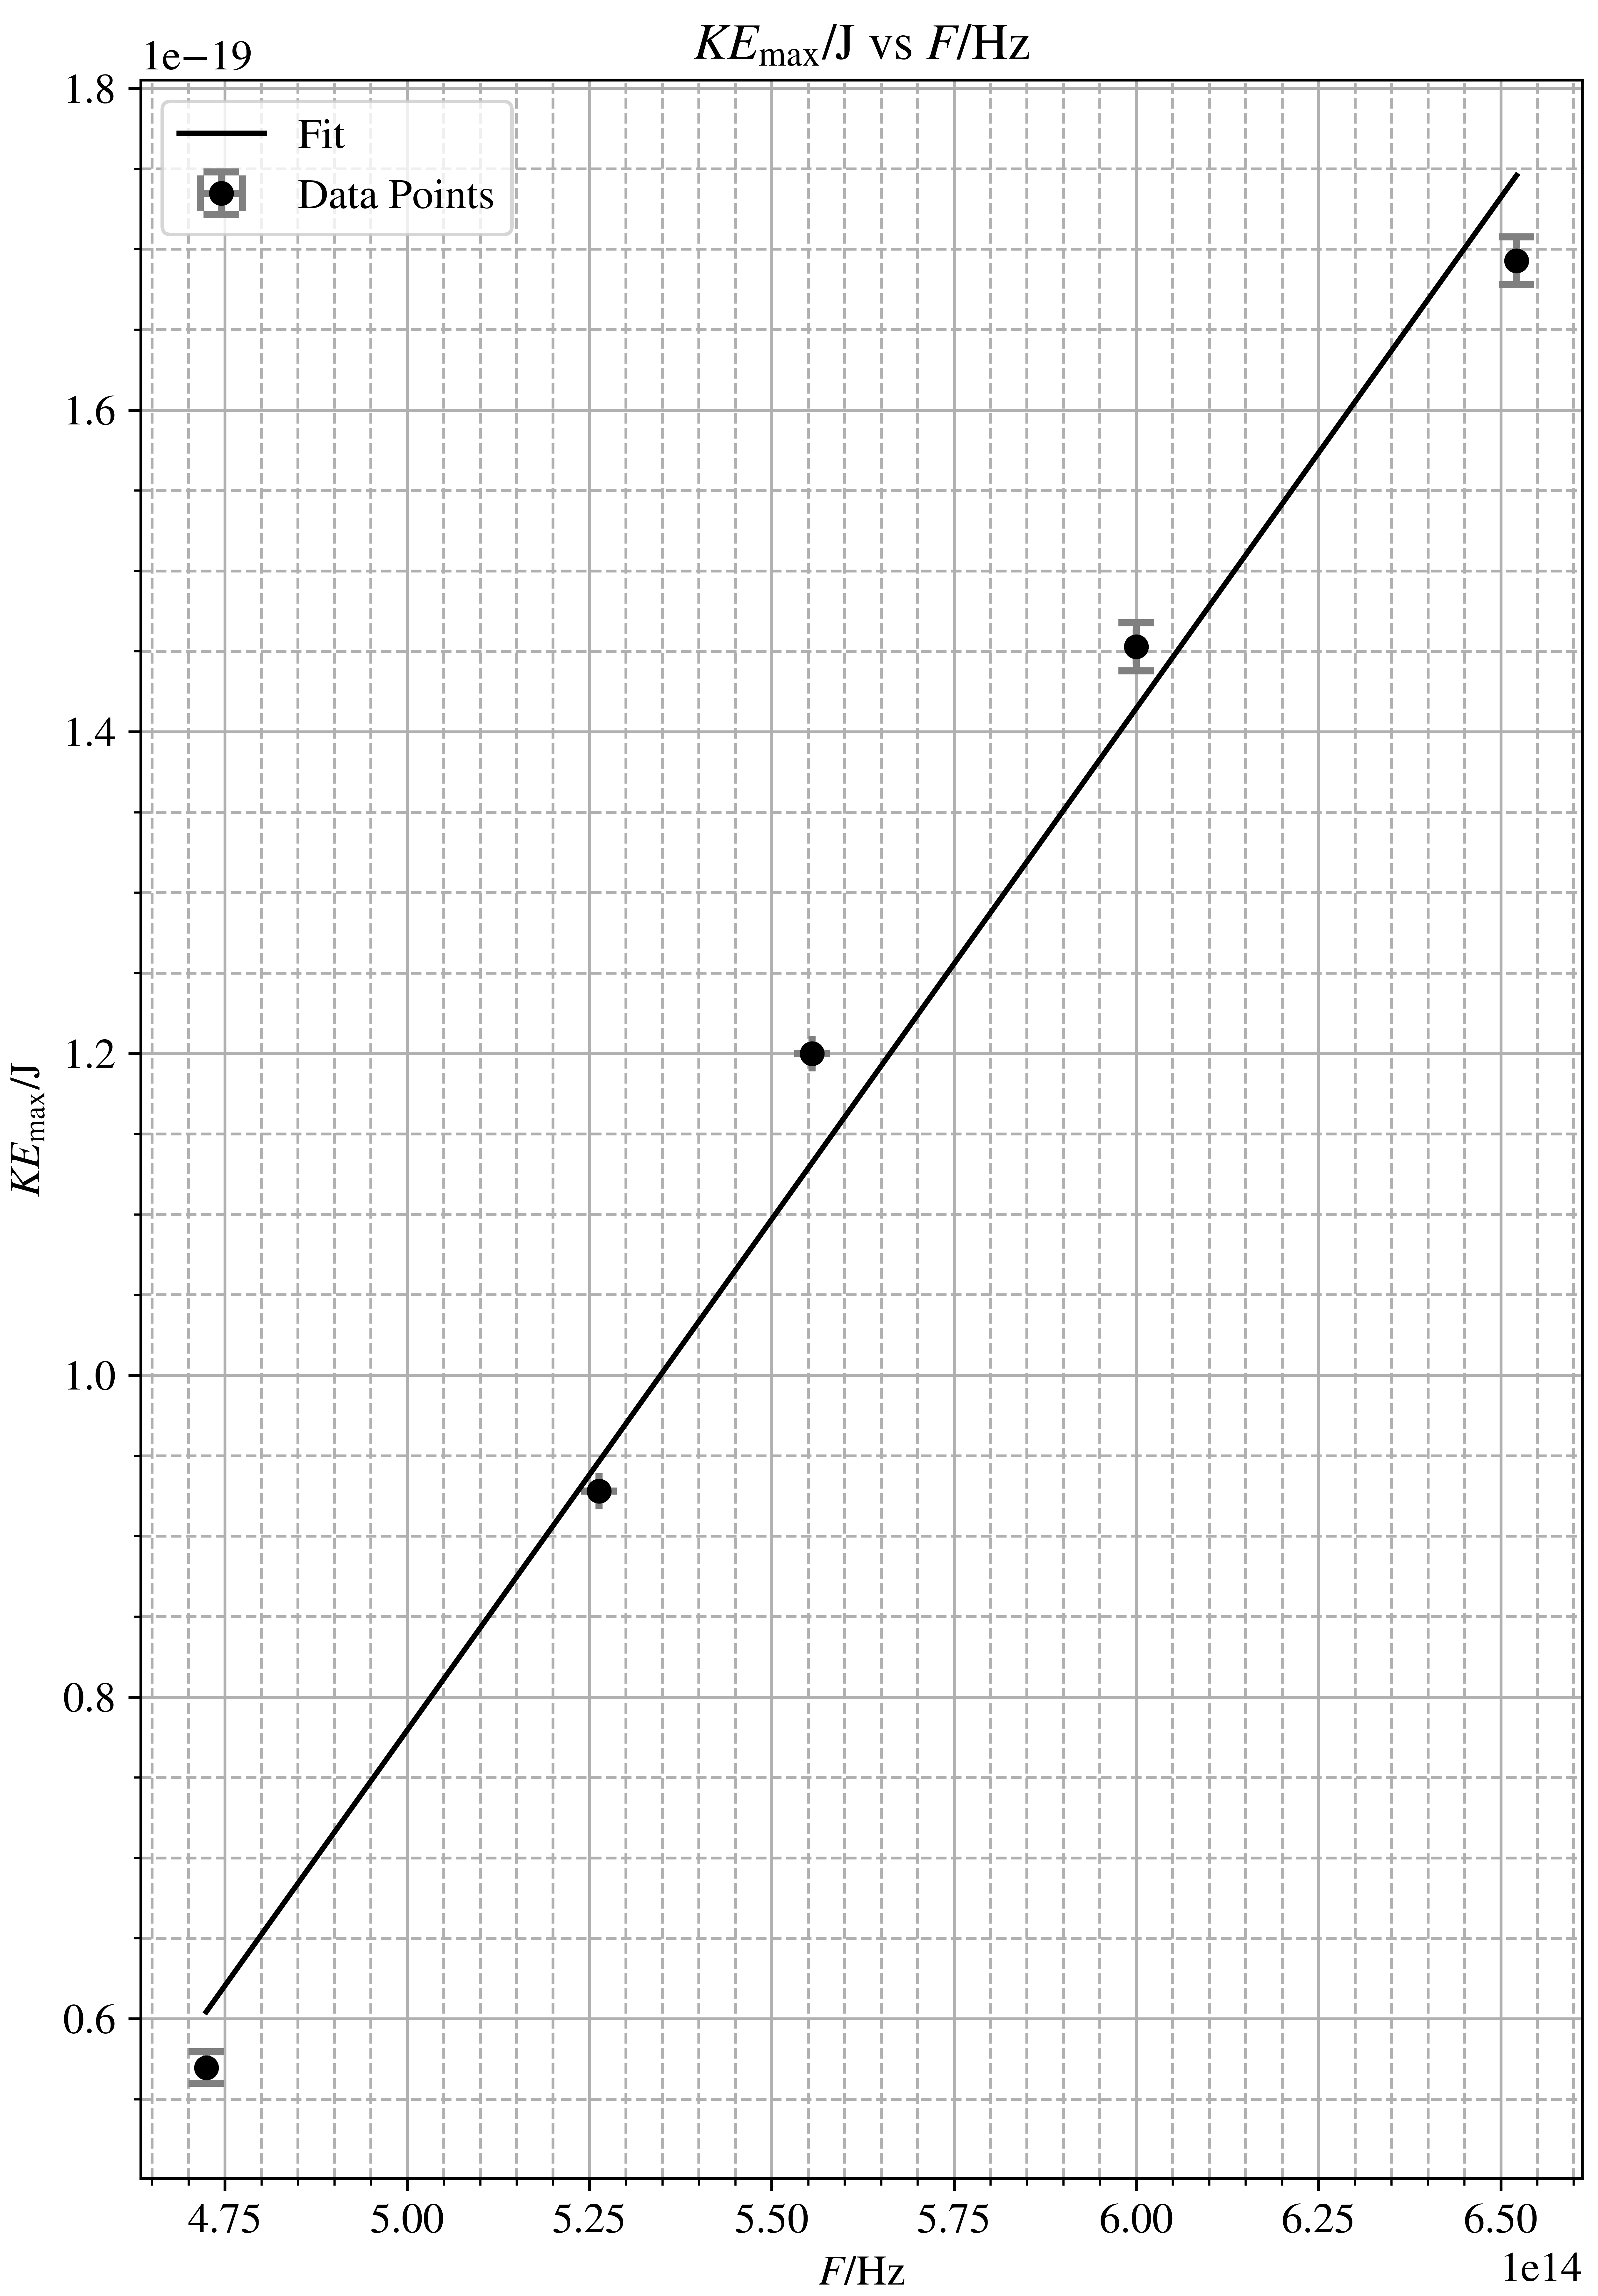
\includegraphics[width=\textwidth]{KEvsFgraph.png}
    \caption{KE$_{\text{max}}$ vs Frequency graph}
    \label{fig:KEvsFgraph}
\end{figure}

\section*{Calculations}
The data collected during the experiment was read by the program using the following line of code:
\begin{lstlisting}
    data = pd.read_excel(`Experiment 15.xlsx').
\end{lstlisting}
The averages of the stopping voltage of each filter was calculated by the program using the following lines of code:
\begin{lstlisting}
    svr = data[`svred'].mean()
    svo = data[`svorange'].mean()
    svy = data[`svyellow'].mean()
    svg = data[`svgreen'].mean()
    svb = data[`svblue'].mean(),
\end{lstlisting}
while the filter wavelengths were imported using the following line of code:
\begin{lstlisting}
    wavelengths = data[`wavelength'].
\end{lstlisting}
As the speed of light and the electron charge are constants they were defined in the program using the following lines of code:
\begin{lstlisting}
    c = 3e8
    e = -1.6e-19.
\end{lstlisting}
The equation given for the experiment that links Planck's constant is:
\begin{equation}
    K E_{\mathrm{max}} = \textrm{h}f + \mathrm{\phi} \,,
\end{equation}
where $K E_{\textrm{max}}$ is the maximum kinetic energy of the electrons, h is Planck's constant, $f$ is the frequency of light, $\mathrm{\phi}$ is the work function of the material. This was compared to the equation of a straight line $y=\text{m} x+\text{c}$. This resulted that the gradient, $\text{m}$, of the straight line corresponds to $h$, and the y-intercept, $\text{c}$, of the straight line corresponds to $\phi$.  $y$ corresponds to $K E_{\textrm{max}}$ and $x$ corresponds to $f$. It was noted that $K E_{\textrm{max}}$ is comparable to the $E$ from $E=m \text{c}^2$, and that E was transformed into $V \text{Q}$ as $E=V \text{Q}$. Also, $f$ was transformed to $\frac{\text{c}}{\lambda}$, as the wave equation is $\text{c}=f\lambda$. Therefore the final equation is:
\begin{equation}
    V \text{Q} = \text{h}\left(\frac{\text{c}}{\lambda}\right) + \mathrm{\phi} \,,
\end{equation}
where $V$ is the voltage, $\text{Q}$ is the electron charge, $\text{c}$ is the speed of light and $\lambda$ is the frequency of the filter. Therefore, $V \text{Q}$, called $K E_{\text{max}}$, against $f$ was plotted, which can be seen in figure \ref{fig:KEvsFgraph}. The line of best fit was obtained using the following lines of code:
\begin{lstlisting}
    coeffs, cov = np.polyfit(frequency, energy, 1, cov=True)
    polyfunc = np.poly1d(coeffs)
    trendline = polyfunc(frequency).
\end{lstlisting}
Using the previous lines of code the correct positions of the ``coeffs" and co-variance matrix were called, with the following lines of code:
\begin{lstlisting}
    m = coeffs[0]
    yint = coeffs[1]
    merr = np.sqrt(cov[0][0])
    yinterr = np.sqrt(cov[1][1]).
\end{lstlisting}
This resulted that Planck's constant is $6.35\times10^{-34} \text{ JHz}^{-1}$ with an error of $4.29\time10^{-35} \text{ JHz}^{-1}$. The work function of the material was found to be $-2.40\times10^{-19} \text{ eV}$ with an error of $2.42\times10^{-20} \text{ eV}$. Next the error bars were plotted by finding $\Delta sv$ using the following equation:
\begin{equation}
    \Delta sv = t_{\alpha, n-1}\, \frac{s}{\sqrt{n}}\,,
\end{equation}
where t is the t-value corresponding to the population number, s is that standard deviation of the values and n is the population size. This was done using the following lines of code:
\begin{lstlisting}
    svstd = np.array([np.std(data[`svred']), np.std(data[`svorange']), 
                  np.std(data[`svyellow']), np.std(data[`svgreen']), 
                  np.std(data[`svblue'])])
    deltasv = np.absolute(e * 2.78 * svstd/np.sqrt(5)).
\end{lstlisting}
The accuracy for Planck's constant was calculated using the following equation:
\begin{equation}
    \text{Accuracy} = \left(\frac{\text{Experiment Value}}{\text{Quoted Value}}-1\right) \times 100\%\,,
\end{equation}
which was done using the following line of code:
\begin{lstlisting}
    maccuracy = np.absolute(((m/6.62e-34)-1) * 100).
\end{lstlisting}
This resulted in an accuracy of $4.06\%$. The precision for both the values of Planck's constant and the work function were found using:
\begin{equation}
    \text{Precision} = \frac{\text{Combined Error}}{\text{Experimental Values}} \times 100 \% \,,
\end{equation}
which was done using the following lines of code:
\begin{lstlisting}
    mprecision = (merr/m) * 100
    yintprecision = np.absolute((yinterr/yint) * 100).
\end{lstlisting}
This resulted in the precision of Planck's constant to be $6.75\%$ and the precision of the work function to be $10.10\%$.

\section*{Discussion}
The aim of this experiment was to determine Planck's constant with the use of the apparatus shown in the diagram \ref{fig:Diagram}. This resulted in the value determined to be $6.35\times10^{-34} \text{ JHz}^{-1}$ \textpm $4.29\times 10^{-35}\text{ JHz}^{-1}$ while the actual value of Planck's constant is $6.62\times10^{-34} \text{ JHz}^{-1}$. This resulted in an accuracy of $4.06\%$, which means that the value obtained was very accurate as it is below the $10\%$ threshold. This level of accuracy is the result of the notable number of precautions taken as mentioned before. With regards to the readings taken during the experiment the combined error of the results obtained for both Planck's constant and the work function of the material were found to be \textpm $4.29\times10^{-35} \text{ JHz}^{-1}$ and \textpm $2.42\times10^{-20} \text{ eV}$ respectively. These values resulted in the precision for both the Planck's constant and the work function to be $6.75\%$ and $10.10\%$ respectively. It should be noted that the value for the precision value of the work function is slightly above the 10\% threshold, which could be due to the sources of error mentioned before. However, the high level of precision can be seen in figure \ref{fig:KEvsFgraph}, as the error bars of each point are relatively small. 

\noindent
The photoelectric effect can be defined as the release of electrons from the surface of a material when light hits its surface \parencite{muncaster}. This phenomenon has been studied extensively, and resulted in many conclusions such as the following:
\begin{enumerate}[label=\roman*.]
    \item Emission only occurs if the frequency of the light used is above a certain threshold, which is called the threshold frequency, and this is dependent on the metal used.
    \item Emission starts immediately as soon as the surface of the metal is hit with light.
    \item The number of electrons emitted per second is proportional to the intensity of the light.
    \item Increasing the frequency of the light increases the energies of the emitted electrons and this increases the maximum kinetic energy.
    \item The intensity of the light has no effect on the kinetic energies of the emitted electrons.
\end{enumerate}
This was shown in the first part of the experiment as the current increased when the bulb was moved closer to the drawtube. This meant that the number of electrons emitted was increased with the higher intensity of light. Also, when the the current was fixed and the stopping voltage was found, the voltage did not fluctuate when the bulb was moved, thus, proving the fact that the light intensity does not effect the kinetic energy. The voltage in this experiment was used to limit the kinetic energy of the electrons in the beginning of the experiment. The photoelectric emission of electrons is used in many applications in real life. One such application is in imaging technology, mainly in older television sets where electrons were used to produce images.  Another use is in the solar cells in photo voltaic cells used to generate energy from the sun, where the photoelectric effect results in the generation of a current \parencite{Photoelectric}.

\printbibliography[title = {References:}]

\section*{Appendix}
\begin{lstlisting}
import numpy as np
import matplotlib.pyplot as plt
import pandas as pd

# importing data from excel and defining constants
data = pd.read_excel(`Experiment 15.xlsx')
svr = data[`svred'].mean()
svo = data[`svorange'].mean()
svy = data[`svyellow'].mean()
svg = data[`svgreen'].mean()
svb = data[`svblue'].mean()

wavelengths = data[`wavelength']
c = 3e8
e = -1.6e-19

energy = np.array([(svr*e), (svo*e), (svy*e), (svg*e), (svb*e)])
frequency = np.array([(c/wavelengths[0]), (c/wavelengths[1]), 
                      (c/wavelengths[2]), (c/wavelengths[3]), 
                      (c/wavelengths[4])])

# finding the change in the stopping voltage
svstd = np.array([np.std(data[`svred']), np.std(data[`svorange']), 
                  np.std(data[`svyellow']), np.std(data[`svgreen']), 
                  np.std(data[`svblue'])])
deltasv = np.absolute(e * 2.78 * svstd/np.sqrt(5))

# finding the coefficients and line of best fit
coeffs, cov = np.polyfit(frequency, energy, 1, cov=True)
polyfunc = np.poly1d(coeffs)
trendline = polyfunc(frequency)

# finding the required values and the errors
m = coeffs[0]
yint = coeffs[1]
merr = np.sqrt(cov[0][0])
yinterr = np.sqrt(cov[1][1])

# finding the accuracy and precision
maccuracy = np.absolute(((m/6.62e-34)-1) * 100)
mprecision = (merr/m) * 100
yintprecision = np.absolute((yinterr/yint) * 100)

# printing everything
print(f`Planks constant was found to be: {m}, 
        with and error of {merr}. '
      f`Its accuracy is {maccuracy:.2f}%, 
        and with a precision of {mprecision:.2f}%')
print(f`The work function of the material was 
        found to be {yint}, with an error of {yinterr}. '
      f`Its precision is {yintprecision}%')

# defining the fonts and sizes to be used
plt.rcParams[`font.family'] = `STIXGeneral'
plt.rcParams[`mathtext.fontset'] = `stix'
plt.rcParams[`font.size'] = 12
plt.rcParams[`font.weight'] = `normal'

# defining the plot size
f = plt.figure(figsize=(7.3, 10.7))

plt.errorbar(frequency, energy, xerr=0.01, yerr= deltasv, 
             fmt=`o', color=`k', elinewidth=2, 
             capthick=2, capsize=5, ecolor=`grey', 
             label='Data Points')
plt.plot(frequency, trendline, color=`k', label=`Fit')
plt.minorticks_on()
plt.grid(b=True, which='major', linestyle='-')
plt.grid(b=True, which='minor', linestyle='--')
plt.xlabel(r'$F$/Hz')
plt.ylabel(r'$KE_{\mathrm{max}}$/J')
plt.title(r'$KE_{\mathrm{max}}$/J vs $F$/Hz')
plt.legend()
plt.savefig('KEvsFgraph.png', dpi=800)
plt.show()
\end{lstlisting}
\end{document}
